\section{周期信号的频谱}

\subsection{周期信号频谱的概念}

对于傅里叶级数$f(t) = \frac{A_0}{2}+\sum\limits_{n=1}^{\infty}A_n\cos(n\Omega t+ \varphi_n)$

\begin{Figure}[振幅频谱]
    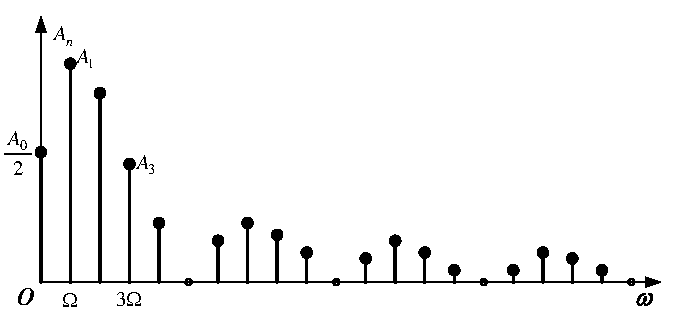
\includegraphics[width=100mm]{visio/4.3.pdf}
\end{Figure}

振幅频谱为$A_n\sim\omega$曲线时为单边谱线,$|F_n|\sim\omega$曲线时为双边谱线。

\begin{Figure}[相位频谱]
    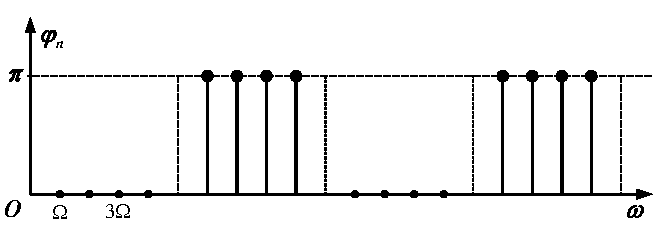
\includegraphics[width=100mm]{visio/4.4.pdf}
\end{Figure}

求某傅里叶级数的频谱图,先求出其基波角频率,再根据各次谐波分量作图。

求某傅里叶级数的双边频谱图,先化为指数形式,写出$F_n$各值再做图。

\subsection{周期信号频谱的特点}

以幅度为$1$,脉冲宽度为$\tau$的周期矩形脉冲为例,其周期为$T$

\begin{Figure}[周期矩形脉冲]
    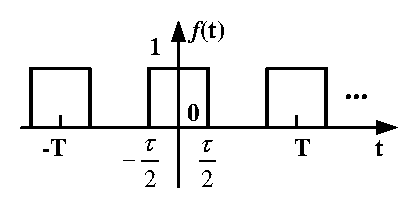
\includegraphics[width=40mm]{visio/4.5.pdf}
\end{Figure}

其频谱$F_n$满足

\begin{Equation}
    F_n=\frac{1}{T}\int_{-\frac{T}{2}}^{\frac{T}{2}}f(t)e^{-\mathrm{j}n\Omega t}dt=\frac{1}{T}\int_{-\frac{\tau}{2}}^{\frac{\tau}{2}}e^{-\mathrm{j}n\Omega t}dt=\frac{1}{T}\left.\frac{e^{-\mathrm{j}n\Omega t}}{-\mathrm{j}n\Omega}\right|^{\frac{\tau}{2}}_{-\frac{\tau}{2}}=\frac{\tau}{T}\frac{\sin\frac{n\Omega\tau}{2}}{\frac{n\Omega\tau}{2}}
\end{Equation}

令$Sa(x)=\frac{\sin(x)}{x}$(取样函数),则

\begin{Equation}
    F_n=\frac{\tau}{T}Sa(\frac{n\Omega\tau}{2})=\frac{\tau}{T}Sa(\frac{n\pi\tau}{T}),n=0,\pm 1,\pm 2,\dots
\end{Equation}

设$T=5\tau$,则

\begin{Figure}[周期矩形脉冲的幅频曲线]
    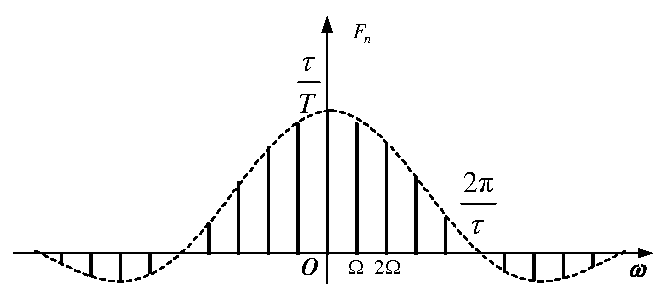
\includegraphics[width=80mm]{visio/4.6.pdf}
\end{Figure}

特点:
\begin{itemize}
    \item 周期信号的频谱具有谐波(离散)性,谱线位置是基频$\Omega$的整数倍
    \item 频谱一般具有收敛性,总趋势减小
    \item $T$一定时,$\tau$变小,此时$\Omega=\frac{2\pi}{T}$(谱线间隔)不变,但两零点间谱线数目$\frac{\omega_1}{\Omega}=\frac{\frac{2\pi}{\tau}}{\frac{2\pi}{T}}=\frac{T}{\tau}$增多
    \item $\tau$一定时,$T$增大,间隔$\Omega$减小,频谱变密,幅度减小($T\rightarrow\infty$时,谱线间隔趋于零,过渡到非周期信号的连续频谱,各频率分量幅度趋于无穷小)
\end{itemize}


\subsection{频带宽度}

由频谱的收敛性可知,信号的功率集中在低频段。

\begin{BoxFormula}[部分功率公式]
    \begin{Equation}
        P_{in}=F_0^2+|F_1|^2+\dots+|F_{i-1}|^2+|F_{-1}|^2+\dots+|F_{-(i-1)}|^2
    \end{Equation}
\end{BoxFormula}

\begin{BoxDefinition}[频带宽度]
    在满足一定失真条件下,信号可以用某段频率范围内的信号表示,此频率范围称为频率宽度。

    对于矩形脉冲信号一般把第一个零点作为信号的频带宽度,记为
    \begin{Equation}
        B_\omega = \frac{2\pi}{\tau}
    \end{Equation}
    或
    \begin{Equation}
        B_f = \frac{1}{\tau}
    \end{Equation}
    带宽与脉宽成反比。
    
    对于一般的周期信号,将幅度下降为$0.1|F_n|_{\mathrm{max}}$的频率区间定义为频带宽度。

    系统的通频带$>$信号的带宽时,信号才不失真。
\end{BoxDefinition}
